\section{Backend}

\subsection{Overview}
The backend of FlowX uses a microservices architecture for scalability and modularity. It consists of:
\begin{itemize}
\item \textbf{API Microservice}: Handles authentication, workflow, and state management.
\item \textbf{Executor Microservice}: Executes LangChain logic.
\item \textbf{Infrastructure Service}: Manages deployment with Terraform and Kubernetes.
\end{itemize}

The following figure shows the API schema for the backend that allows Workflow creation:
\begin{figure}[H]
    \centering
    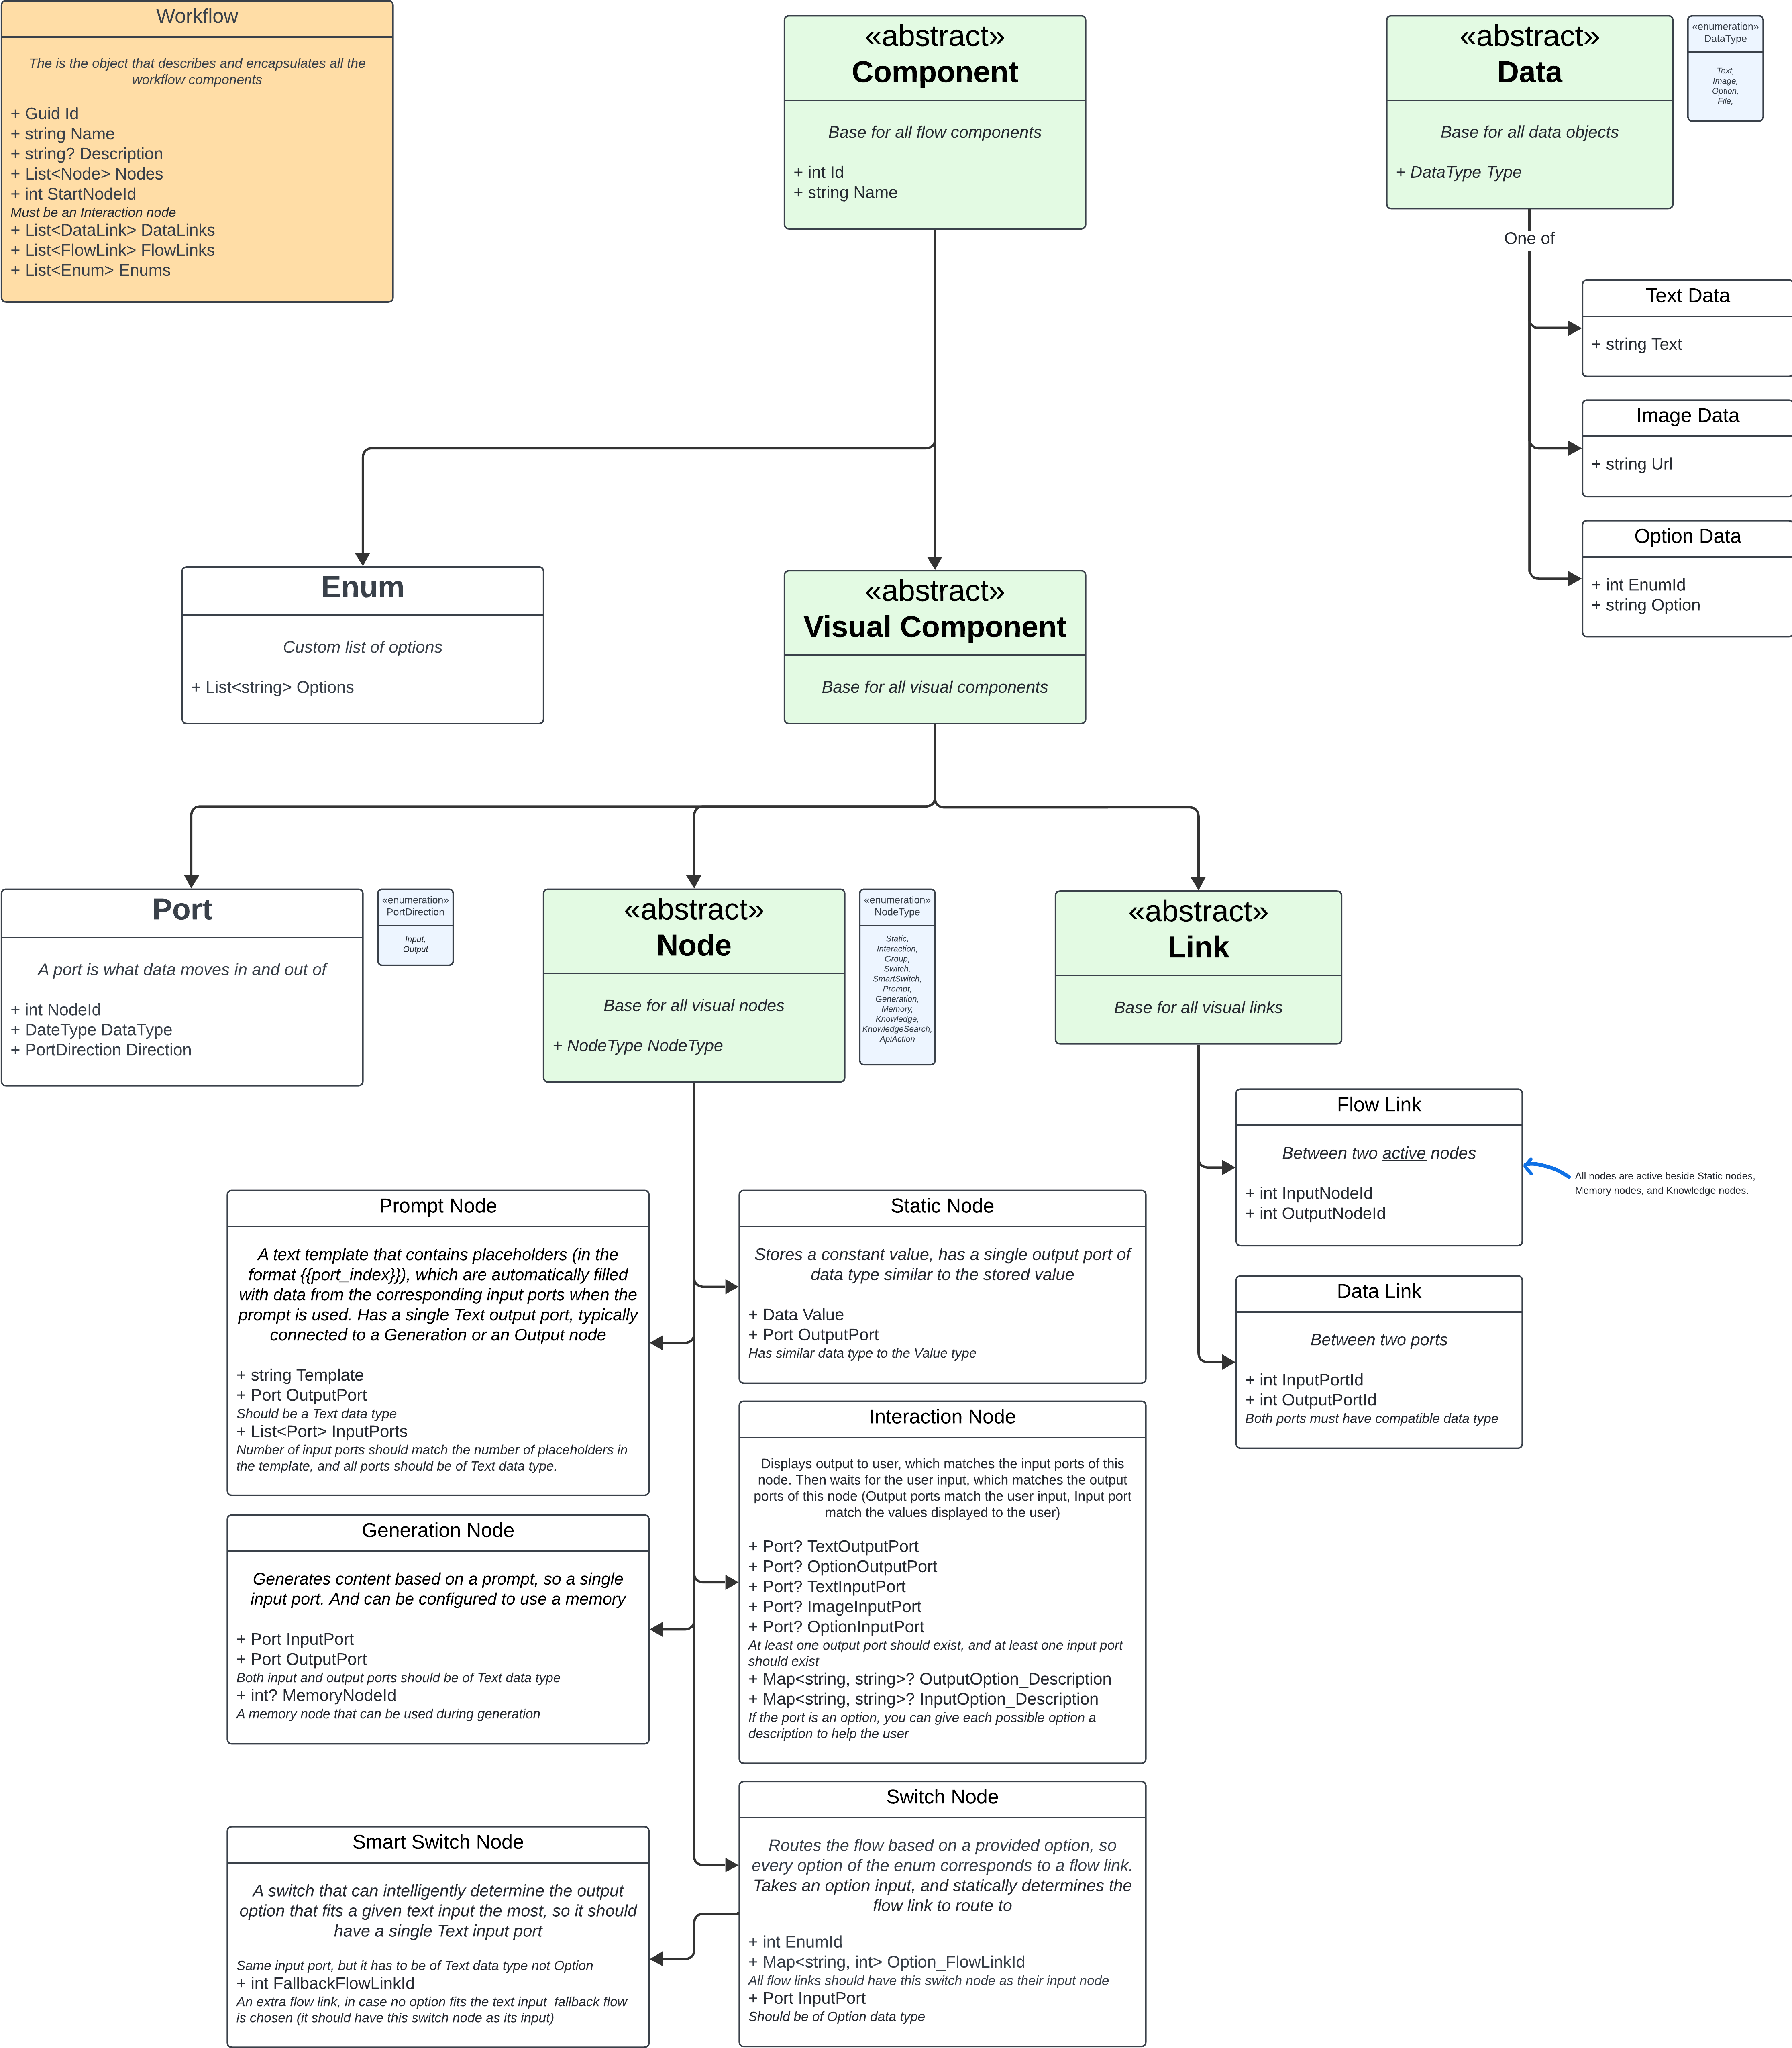
\includegraphics[width=0.95\textwidth]{assets/ChatbotBuilderApiSchema}
    \caption{API Schema for Chatbot Builder Workflows}
    \label{fig:api_schema}
\end{figure}

\subsection{API Microservice}
Built with \textbf{ASP.NET Core}, this service handles:
\begin{itemize}
\item \textbf{Authentication}: Uses JWT-based security.
\item \textbf{Workflow Management}: Supports CRUD operations.
\item \textbf{State Management}: Tracks chatbot workflow states.
\item \textbf{Executor Communication}: Delegates execution via gRPC.
\end{itemize}



\subsection{Executor Microservice}
Developed in \textbf{Python} with \textbf{LangChain}, responsible for:
\begin{itemize}
\item \textbf{Chatbot Logic Execution}.
\item \textbf{gRPC Communication} with the API service.
\item \textbf{Handling Smart Switch Nodes} using LLM outputs.
\end{itemize}

\subsection{Infrastructure and Deployment}
Managed using \textbf{Terraform} and \textbf{Kubernetes}, ensuring:
\begin{itemize}
\item \textbf{Scalable Deployment}: Kubernetes handles scaling and failover.
\item \textbf{Infrastructure as Code (IaC)}: Terraform automates provisioning.
\item \textbf{Service Communication}: Uses gRPC and RESTful APIs.
\end{itemize}